%% Qualitative results on the ground-truth retrieval benchmark (two columns).
%% The graphic is a 5 x 6 matrix of images -- 5 touch locations (rows) x 6 streams (columns):
%%   1. reference touch, middle frame
%%   2. reference normal render at the reference sensor pose
%%   3. query normal render at the query sensor pose
%%   4. query touch, coarse transfer
%%   5. query touch, refined transfer (ours)
%%   6. ground-truth query touch
%% Columns 2 and 3 show four times the sensor footprint with the sensor's own footprint
%% boxed in red, are drawn on white, and are the only columns with an outline.
%% Graphic: figures/gt_retrieval.png
%% Column headers are baked into the image.
%% Source PDF: log/paper_job06_gt_retrieval_figure/gt_retrieval.pdf (white page, black text)
%% Per-cell PNGs: log/paper_job06_gt_retrieval_figure/assets_pdf/gt_retrieval/
%%   rowN_<object>_<touch>_colM_<stream>.png
%% Rows shown: objects 974/5, 978/4, 969/3, 970/7, 995/5.
%% Built by paper_experiments/06_gt_retrieval_figure/make_gt_figure.py; per-cell PNGs for
%% all 400 evaluation touches remain in
%%   log/paper_job02_gt_retrieval_figure_normalmatch/assets/
%%   named <object>_<touch>_01_ref_touch.png ... _06_gt_query.png
\begin{figure*}[t]
  \centering
  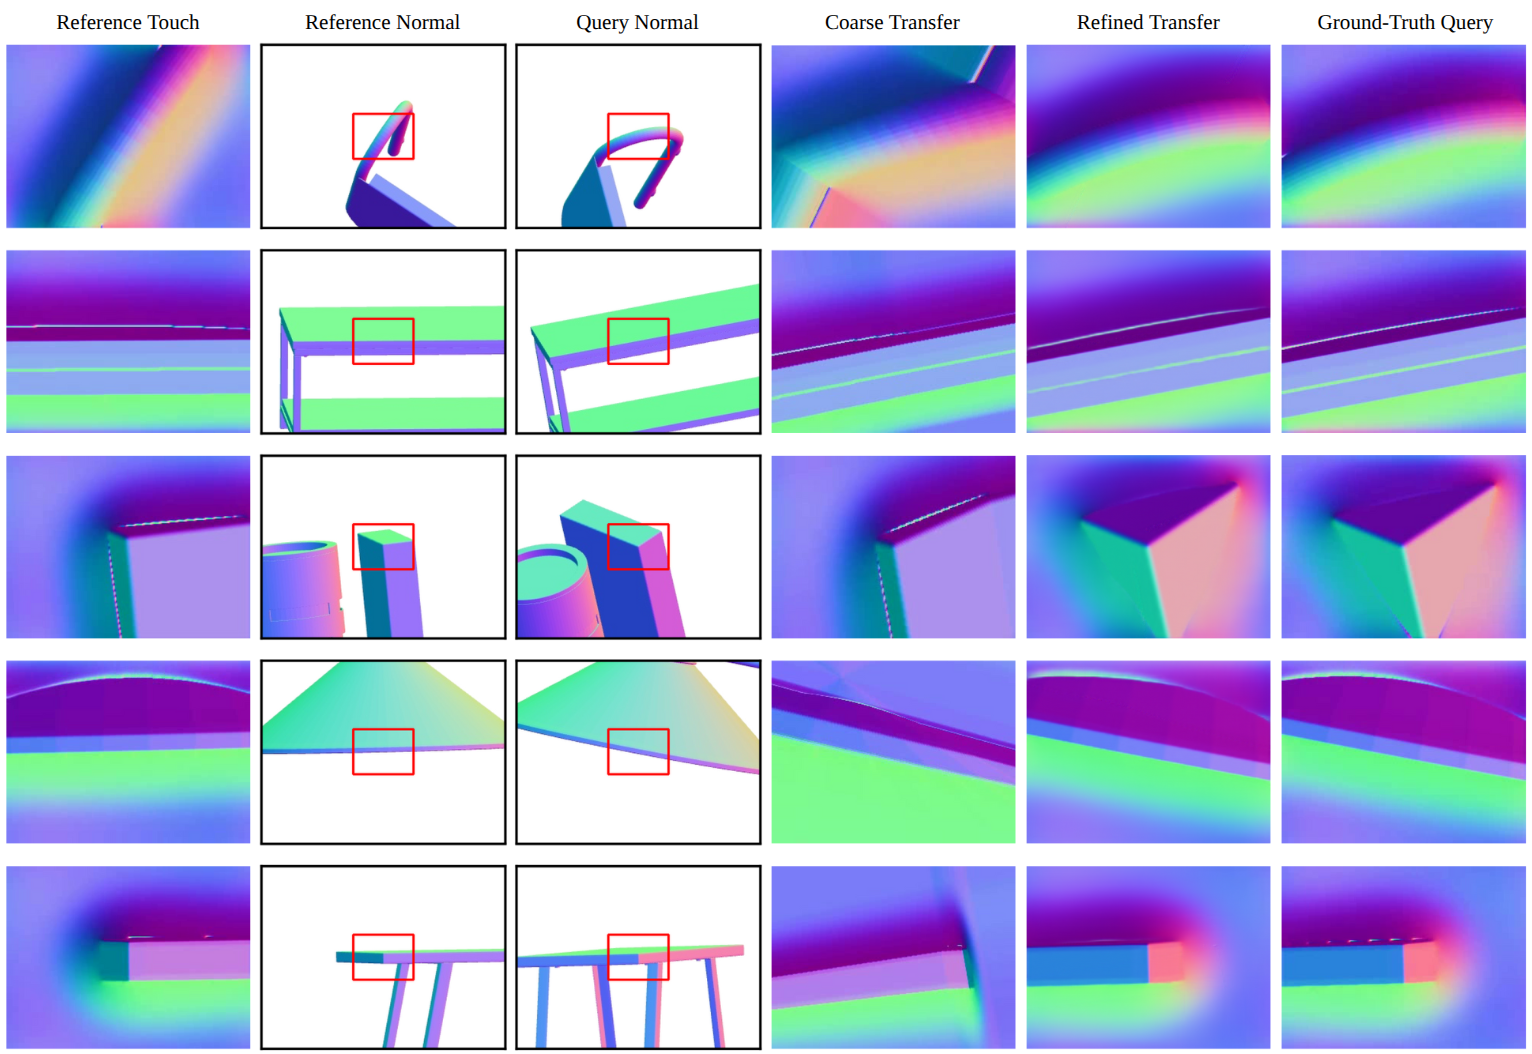
\includegraphics[width=\linewidth]{figures/gt_retrieval.png}
  \caption{\textbf{Qualitative results on the ground-truth retrieval benchmark.} Each row is one
    touch location. From left to right: the reference touch, the surface normal render at the
    reference sensor pose, the surface normal render at the query sensor pose, the coarse transfer
    obtained by warping the reference touch through the estimated homography, our refined
    prediction, and the ground-truth touch at the query location. The two normal renders cover
    four times the sensor footprint, which is the field of view the correspondences are computed
    at, and the red box marks the patch the sensor itself covers. All tactile frames are the
    middle frame of the 50-frame press, which is also the deepest-contact frame. The refinement
    network sharpens the contact boundary and corrects residual misalignment left by the coarse
    step.}
  \label{fig:gt_retrieval}
\end{figure*}
